\documentclass[11pt]{article}

% ----- lightweight preamble -----
\usepackage[a4paper,margin=2cm]{geometry}
\usepackage{amsmath,amssymb}
\usepackage{tikz}
\usepackage{tikz-cd}
\usetikzlibrary{arrows.meta,positioning,calc,fit,backgrounds}
\usepackage[most]{tcolorbox}
\usepackage{parskip}
\usepackage{xcolor}

\definecolor{gold}{RGB}{200,140,0}
\definecolor{kas}{RGB}{30,110,190}
\definecolor{ink}{RGB}{40,40,40}
\definecolor{soft}{RGB}{245,245,248}

\newtcolorbox{note}[1][]{colback=soft,colframe=ink,boxrule=0.4pt,
  arc=2pt,left=6pt,right=6pt,top=4pt,bottom=4pt,#1}

\tikzset{
  obj/.style={draw=ink,rounded corners=3pt,fill=soft,inner sep=5pt,font=\small},
  gnode/.style={circle,draw=gold,fill=gold!12,minimum size=8mm,font=\small},
  knode/.style={circle,draw=kas,fill=kas!12,minimum size=8mm,font=\small},
  arr/.style={-{Stealth[length=2.5mm]},thick},
}

\title{\vspace{-1.5cm}\textbf{Conjugacy Exploration --- a picture book}\\[2pt]
\large Frobenius shift, intertwiners, and the Gold\,/\,Kasami test}
\author{\small Visual summary of \texttt{Dobbertin1999MVP/ShiftConjugacy.lean}}
\date{}

\begin{document}
\maketitle
\vspace{-1.2cm}

\begin{note}
\textbf{One line.} Kasami and Gold are \emph{not} the same map up to a
Frobenius shift. The real bridge is a bigger kind of map (an
\emph{intertwiner}). Every claim below is machine-checked in Lean.
\end{note}

%======================================================================
\section*{1. The players: a set with a self-map}

An \textbf{object} is a set with one arrow going back into itself.

\begin{center}
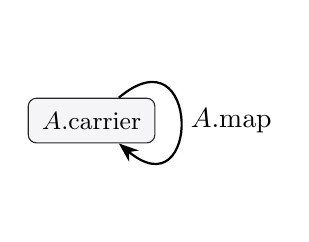
\begin{tikzpicture}
  \node[obj] (A) {$A.\mathrm{carrier}$};
  \draw[arr] (A) to[out=40,in=-40,looseness=6] node[right]{$A.\mathrm{map}$} (A);
\end{tikzpicture}
\end{center}

A \textbf{morphism} $L:A\to B$ is a map that \emph{respects} the self-maps.
The square commutes: go right-then-down $=$ go down-then-right.

\begin{center}
\begin{tikzcd}[column sep=large,row sep=large]
A.\mathrm{carrier} \arrow[r,"L"] \arrow[d,"A.\mathrm{map}"'] &
B.\mathrm{carrier} \arrow[d,"B.\mathrm{map}"] \\
A.\mathrm{carrier} \arrow[r,"L"'] &
B.\mathrm{carrier}
\end{tikzcd}
\end{center}

\begin{center}\small
Lean: \texttt{structure Endo}, \texttt{structure EndoHom} with law
$B.\mathrm{map}\,(L\,x)=L\,(A.\mathrm{map}\,x)$.\\
These objects and arrows form a category (\texttt{instance : Category Endo}).
\end{center}

%======================================================================
\section*{2. Conjugacy $=$ isomorphism}

If $L$ is a \textbf{bijection} then the arrow flips for free: $L^{-1}$ is
again a morphism. So a two-way arrow means the two self-maps are
\textbf{conjugate}.

\begin{center}
\begin{tikzcd}[column sep=huge,row sep=large]
A.\mathrm{carrier}
  \arrow[r,shift left=1.2ex,"L"]
  \arrow[d,"A.\mathrm{map}"'] &
B.\mathrm{carrier}
  \arrow[l,shift left=1.2ex,"L^{-1}"]
  \arrow[d,"B.\mathrm{map}"] \\
A.\mathrm{carrier}
  \arrow[r,shift left=1.2ex,"L"]  &
B.\mathrm{carrier}
  \arrow[l,shift left=1.2ex,"L^{-1}"]
\end{tikzcd}
$\qquad\Longleftrightarrow\qquad B.\mathrm{map}=L\circ A.\mathrm{map}\circ L^{-1}$
\end{center}

\begin{center}\small
Lean: \texttt{isoOfEquiv} (bijective intertwiner $\Rightarrow$ iso),
\texttt{Conjugate}.\\
The paper's substitution $\psi_\beta$ (MCM $\Leftrightarrow$ Kasami) is one
such isomorphism.
\end{center}

%======================================================================
\section*{3. Frobenius $=$ the shift on exponents}

Take power maps $x\mapsto x^{e}$. On the \emph{exponent} $e$, squaring
($x\mapsto x^{2}$) is just \textbf{doubling} $e\mapsto 2e$.

\begin{center}
\begin{tikzcd}[column sep=huge]
x \arrow[r,"(\,\cdot\,)^{e}"] \arrow[dr,"(\,\cdot\,)^{2e}"'] &
x^{e} \arrow[d,"(\,\cdot\,)^{2}"] \\
& x^{2e}
\end{tikzcd}
\qquad
$x^{2e}=(x^{e})^{2}$
\end{center}

Every Frobenius power $x\mapsto x^{2^{i}}$ is a self-arrow of the object
$x\mapsto x^{e}$ (it slides past the power map):

\begin{center}
\begin{tikzcd}[column sep=huge,row sep=large]
x \arrow[r,"(\,\cdot\,)^{2^{i}}"] \arrow[d,"(\,\cdot\,)^{e}"'] &
x^{2^{i}} \arrow[d,"(\,\cdot\,)^{e}"] \\
x^{e} \arrow[r,"(\,\cdot\,)^{2^{i}}"'] &
(x^{e})^{2^{i}}=(x^{2^{i}})^{e}
\end{tikzcd}
\end{center}

\begin{center}\small
Lean: \texttt{frobenius\_realizes\_shift}, \texttt{frob\_pow\_intertwines},
\texttt{frobPowHom}.
\end{center}

%======================================================================
\section*{4. Orbits of doubling $=$ cyclotomic cosets}

Work mod $m=2^{n}-1$. Doubling $e\mapsto 2e$ marches an exponent around a
cycle. Running $i<n$ gives \emph{all} $n$ field automorphisms of
$\mathbb{F}_{2^{n}}$. Each cycle is a \textbf{cyclotomic coset}.

Example $n=5$, $m=31$. The Gold exponent $5$ walks a 5-cycle:

\begin{center}
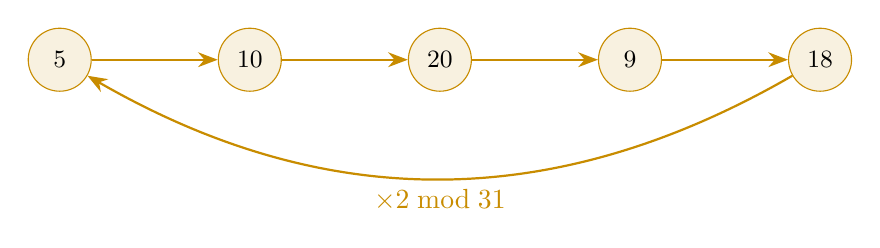
\begin{tikzpicture}[node distance=16mm]
  \node[gnode] (a){$5$};
  \node[gnode,right=of a] (b){$10$};
  \node[gnode,right=of b] (c){$20$};
  \node[gnode,right=of c] (d){$9$};
  \node[gnode,right=of d] (e){$18$};
  \draw[arr,gold] (a)--(b); \draw[arr,gold](b)--(c);
  \draw[arr,gold] (c)--(d); \draw[arr,gold](d)--(e);
  \draw[arr,gold] (e) to[out=-150,in=-30] node[below]{$\times 2 \bmod 31$} (a);
\end{tikzpicture}
\end{center}

%======================================================================
\section*{5. The test: does Gold meet Kasami?}

Gold exponent $2^{k}+1$ \quad vs \quad Kasami exponent $2^{2k}-2^{k}+1$.

\textbf{At $k=1$ they collapse to the same number} ($3$). No genuine Kasami
yet.

\begin{center}
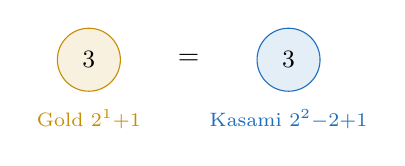
\begin{tikzpicture}
  \node[gnode] (g){$3$};
  \node[right=6mm of g] (eq){$=$};
  \node[knode,right=6mm of eq] (k){$3$};
  \node[below=1mm of g,font=\scriptsize,gold]{Gold $2^1{+}1$};
  \node[below=1mm of k,font=\scriptsize,kas]{Kasami $2^2{-}2{+}1$};
\end{tikzpicture}\\[2pt]
{\small Lean: \texttt{kasami\_eq\_gold\_at\_one}.}
\end{center}

\textbf{At $k\ge 2$ they live in different cycles} --- no amount of doubling
(no Frobenius power) moves one onto the other. Case $n=5,\;k=2$:
Gold\,$=5$, Kasami\,$=13$, mod $31$.

\begin{center}
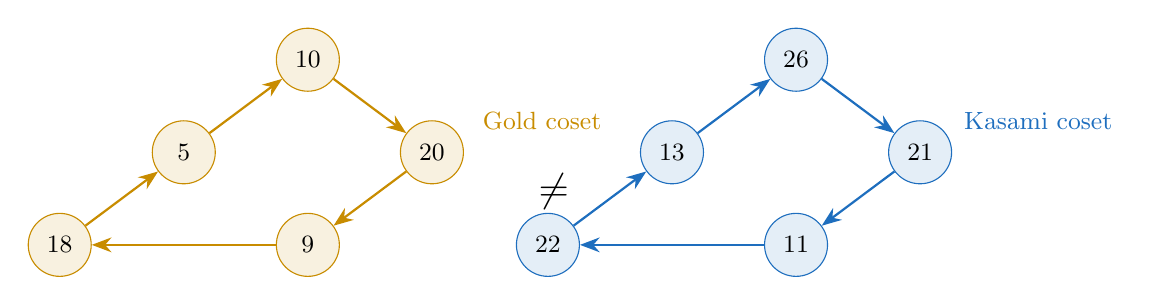
\begin{tikzpicture}[node distance=13mm]
  % Gold cycle
  \node[gnode] (g0){$5$};
  \node[gnode,above right=6mm and 10mm of g0] (g1){$10$};
  \node[gnode,below right=6mm and 10mm of g1] (g2){$20$};
  \node[gnode,below left=6mm and 10mm of g2] (g3){$9$};
  \node[gnode,below left=6mm and 10mm of g0] (g4){$18$};
  \draw[arr,gold](g0)--(g1);\draw[arr,gold](g1)--(g2);
  \draw[arr,gold](g2)--(g3);\draw[arr,gold](g3)--(g4);
  \draw[arr,gold](g4)--(g0);
  \node[gold,font=\small] at ($(g2)+(1.4,0.4)$){Gold coset};

  % Kasami cycle, shifted right
  \begin{scope}[xshift=6.2cm]
  \node[knode] (k0){$13$};
  \node[knode,above right=6mm and 10mm of k0] (k1){$26$};
  \node[knode,below right=6mm and 10mm of k1] (k2){$21$};
  \node[knode,below left=6mm and 10mm of k2] (k3){$11$};
  \node[knode,below left=6mm and 10mm of k0] (k4){$22$};
  \draw[arr,kas](k0)--(k1);\draw[arr,kas](k1)--(k2);
  \draw[arr,kas](k2)--(k3);\draw[arr,kas](k3)--(k4);
  \draw[arr,kas](k4)--(k0);
  \node[kas,font=\small] at ($(k2)+(1.5,0.4)$){Kasami coset};
  \end{scope}

  % separation
  \node at (4.7,-0.5){\Large$\neq$};
\end{tikzpicture}
\end{center}

\begin{center}\small
Two disjoint cycles $\Rightarrow$ no Frobenius power links them. Checked for\\
$(n,k)=(5,2),(7,2),(7,3),(11,2),(13,3)$:
\texttt{gold\_kasami\_not\_frobEquiv\_*}.
\end{center}

%======================================================================
\section*{6. Bonus: the \emph{same} shift, put to work (even $k$)}

The conjugacy exploration says Frobenius \textbf{cannot} link two
\emph{different} cosets (Gold vs Kasami). The flip side: when two exponents
sit in the \emph{same} coset, Frobenius links them for free --- and that is
exactly the trick that removes the ``$k$ odd'' restriction from Kasami APN.

Kasami with parameter $k$ and with parameter $n-k$ live in \textbf{one}
coset:
\[
  d_k \;=\; d_{\,n-k}\cdot 2^{2k} \pmod{2^{n}-1},
  \qquad\text{so}\qquad
  x^{d_k} \;=\; \big(x^{d_{\,n-k}}\big)^{2^{2k}}
  \;=\; \mathrm{Frob}_{2k}\!\big(x^{d_{\,n-k}}\big).
\]

\begin{center}
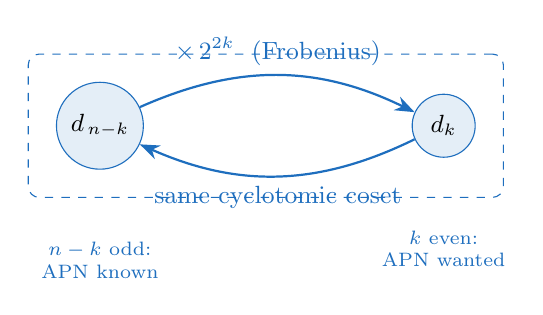
\begin{tikzpicture}[node distance=34mm]
  \node[knode] (a){$d_{\,n-k}$};
  \node[knode,right=of a] (b){$d_{k}$};
  \draw[arr,kas] (a) to[bend left=25]
     node[above,font=\small]{$\times\,2^{2k}$ \ (Frobenius)} (b);
  \draw[arr,kas] (b) to[bend left=25]
     node[below,font=\small]{same cyclotomic coset} (a);
  \node[below=8mm of a,font=\scriptsize,kas,align=center]{$n-k$ odd:\\APN known};
  \node[below=8mm of b,font=\scriptsize,kas,align=center]{$k$ even:\\APN wanted};
  \begin{scope}[on background layer]
    \node[draw=kas,dashed,rounded corners,fit=(a)(b),inner sep=10pt]{};
  \end{scope}
\end{tikzpicture}
\end{center}

Frobenius is an additive bijection, so it \textbf{preserves APN}. Transfer
from the odd side ($n-k$) to the even side ($k$). Done.

\begin{center}\small
Lean: \texttt{kasami\_pow\_frob\_identity}, \texttt{apn\_frob\_twist},
\texttt{kasami\_apn\_of\_complement}, \texttt{kasami\_is\_apn\_general}\\
(and \texttt{IsAPN.comp\_frobenius} in the differential-uniformity library).
\end{center}

\begin{note}
\textbf{Does Dobbertin use this move? Yes --- word for word.} Right after
Corollary~2 he writes: \emph{``we may assume that $k$ is odd without loss of
generality. (In fact, replace $k$ by $n-k$ if $k$ is even. This replacement
does not change the APN property.)''} His justification is
\emph{cyclotomic equivalence} --- his ``cyclic shift'' is our Frobenius shift.
The same $k\leftrightarrow n-k$ symmetry reappears for his difference sets:
\emph{``$B$ does not change if $(k,k')$ is replaced by $(n-k,n-k')$.''}
\end{note}

\begin{note}
\textbf{How it relates to the MCM\,$\Leftrightarrow$\,Kasami bridge.} Two
different uses of \emph{one} idea (conjugacy in the category of
self-maps):
\begin{itemize}\itemsep0pt
  \item \textbf{Inside} a coset ($k\leftrightarrow n-k$): the intertwiner
    \emph{is} a Frobenius power. Cheap, and it patches the parity gap so the
    MCM proof (which needs $k$ odd) covers \emph{all} $k$.
  \item \textbf{Across} cosets (MCM\,$\Leftrightarrow$\,Kasami, $\psi_\beta$):
    the intertwiner is additive but \emph{not} Frobenius --- the exploration
    shows Frobenius alone cannot do it.
\end{itemize}
So the Frobenius twist is the \emph{complement} of $\psi_\beta$, not a
rival: it is the special (same-coset) case of the same conjugacy umbrella.
\end{note}

%======================================================================
\section*{7. Verdict}

\begin{center}
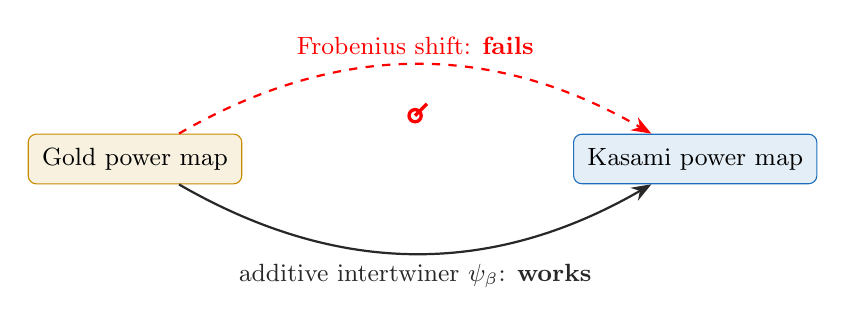
\begin{tikzpicture}[node distance=9mm]
  \node[obj,fill=gold!12,draw=gold] (G){Gold power map};
  \node[obj,fill=kas!12,draw=kas,right=42mm of G] (K){Kasami power map};
  % no frobenius
  \draw[arr,red,dashed] (G) to[bend left=30]
     node[above,font=\small,red]{Frobenius shift: \textbf{fails}} (K);
  \draw[red,very thick] ($(G)!0.5!(K)+(0,0.55)$) circle(2.2pt)
     ($(G)!0.5!(K)+(0,0.55)$) -- ++(0.15,0.15);
  % intertwiner works
  \draw[arr,ink] (G) to[bend right=30]
     node[below,font=\small]{additive intertwiner $\psi_\beta$: \textbf{works}} (K);
\end{tikzpicture}
\end{center}

\begin{note}
The shift picture is the right \emph{idea}, but the umbrella map is a
genuine morphism of the conjugacy category --- an additive (linearized)
intertwiner --- \textbf{not} a power of Frobenius.
\end{note}

\vfill
\begin{center}\scriptsize
All statements verified \texttt{sorry}-free in Lean\,/\,Mathlib.
Source: \texttt{Dobbertin1999MVP/ShiftConjugacy.lean}.
\end{center}

\end{document}
